\documentclass[11pt, oneside]{article}   	% use "amsart" instead of "article" for AMSLaTeX format
\usepackage[a4paper]{geometry}                		% See geometry.pdf to learn the layout options. There are lots.
\geometry{letterpaper}   
%\geometry{left=2.5cm,right=2.5cm,top=2.5cm,bottom=2.5cm}                   		% ... or a4paper or a5paper or ... 
%\geometry{landscape}                		% Activate for rotated page geometry
%\usepackage[parfill]{parskip}    		% Activate to begin paragraphs with an empty line rather than an indent
\usepackage{graphicx}				% Use pdf, png, jpg, or eps§ with pdflatex; use eps in DVI mode
								% TeX will automatically convert eps --> pdf in pdflatex		
\usepackage{amssymb}
\usepackage{appendix}
\usepackage{subfigure}
\usepackage{ulem}
\usepackage{booktabs}
\usepackage{adjustbox}
\usepackage{pifont}

\usepackage{color}
\usepackage{url}

%SetFonts

%SetFonts


\title{\bf How AI can advances the building of Domain Specific Languages ?}
\author{Gabriela Garcia Romero, Willem Nicolas, Akina Renard, Suhairi Subhi and Amine Yahemdi }
\date{}							% Activate to display a given date or no date

\begin{document}
\maketitle

{\noindent\small{\bf Abstract:} TBC}

\vspace{1ex}
{\noindent\small{\bf Keywords:}
   TBC}



\section{Introduction}


\section{Background}

\subsection{Model Driven Engineering}
Model-driven engineering (MDE) is a software development approach that focuses on creating and using domain-specific models as the main artifacts for software development. These models are used to represent the different aspects of the software system, such as its functionality, behavior, structure, and data. MDE aims to provide a higher level of abstraction for software development, allowing developers to focus on the problem domain rather than on the technical details of the implementation\cite{methodologyBasedMDE}..

MDE is based on the idea that models can be transformed into different representations, such as code, configuration files, or documentation. This process is supported by model transformation techniques, which are used to transform the models into the desired representations.

One of the main benefits of MDE is that it allows developers to work with domain-specific languages (DSLs). DSLs are specialized languages that are tailored to a particular problem domain. They allow developers to express the concepts and rules of the domain in a more concise and intuitive way, making it easier to understand and manipulate the models.
There are different types of DSLs, ranging from visual languages \cite{designDSLandIDEforIOTa}, such as UML diagrams, to textual languages, such as regular expressions. Each type of DSL has its own advantages and disadvantages, and the choice of a particular DSL depends on the specific needs of the project.

In addition to simplifying the development process, MDE and DSLs can also improve the quality and maintainability of the software. By using models as the main artifacts, developers can better capture the intended behavior and structure of the system\cite{MDE4IOT}, making it easier to understand and modify the software. This can reduce the number of defects and improve the overall reliability of the system.

In summary, MDE and DSLs provide a powerful toolset for software development, allowing developers to work at a higher level of abstraction and to focus on the problem domain rather than on the technical details. By using models and domain-specific languages, developers can create more reliable and maintainable software systems that are easier to understand and modify.

\subsection{Domain Specification Language:}

A Domain Specific Language (DSL) is a computer language that has constructs and notations tailored to a specific application domain \cite{DSL}, contrary to General Purpose Languages (GPLs) which are applicable across several domains. These constructs and notations offer substantial gains in expressiveness, eases the programing understanding and reduces the semantic distance to the domain in question \cite{DSLwhenwhere}. They can also give tools to perform analysis, verification, optimization, and error checking thar GPLs can’t offer to the given domain.

There are two types of DSLs, internal and external DSLs \cite{usabilityDSL}. Firstly, the internal DSLs which are an extension of core language, usually a GPLs, which offers specific functionalities over the core language syntax.  On the other hand, external DSLs, that are completely independent from the core language, offer their own syntactic and semantic structures, and have their own parser, interpreter, or compiler.

The utilization of DSLs leads to a new paradigm of programing called Language-Oriented programing, in which engineering problems are solved by creating a DSLs that are able to describe the problem and give the solution to it. By creating a new language, the solution will be more reliable, portable, and reusable in other problems of the same domain.

DSLs can be closely related to MDE. Not only there are some DSLs such as UML and SysML that are used to model systems and from there generate software components through generative programming. But also, DSLs can be themselves artifacts for MDE, as they are metamodels for the domain in question, that describe classes, attributes, datatypes, and their relations. From there, it is possible to adapt this metamodel to specify more refined systems in the domain.




\subsection{Artificial Intelligence} 
Artificial intelligence has been an interesting domain in this era, allowing developers and others to benefit from its capacity. Although this domain is usually vast, its current branch called Machine Learning(ML) has seen a rise in popularity. Machine learning uses statistical modelling and computational learning technology in order to recognise pattern in a given datasets. All the ML existing techniques can be divided into several categories based on its different characteristic: frequency of learning, nature of learning, etc.

For the frequency of learning, we can divide the ML techniques into two categories, online and offline learning. Online Learning uses real time input and output to incrementally modify its state for each observation. However in an offline learning, a batch of this observations are sent to the model from time to time.

Nonetheless, ML techniques can also be recognized from its different nature of learning. In this category, the ML techniques are called supervised and unsupervised learning. A supervised learning differs from unsupervised learning in terms of the pre-recognition of the labels or classed that can be found in the datasets, such as regression or classification. The unsupervised techniques starts the learning process with zero knowledge of the data, constructing the labels in the dataset one step after another, where the clustering technique is the mostly wide used. 

The challenges in using Artificial Intelligence(or more precisely Machine Learning) in Model-Driven Engineering is due to the lack of datasets that the ML models can learn from. Even if the datasets are available, the heterogenous nature of the datasets specifically for the Internet of Things(IoT) technologies are delimiting the application of AI techniques in the domain. The learning granularity of the AI models needs to be fine-grained in order to obtain a more accurate and efficient learning.

The different notions of models in AI and MDE also brings some difficulty in integrating these two domain together. ML models or techniques as mentioned above are completely distinct than the models used in MDE; one is a statistical model while another is a structural model. Various works such as ML-Quadrat are looking forward to create a synergy between this models, allowing a more seamless model engineering in the domain.

\subsection{IoT Definition : }
%Do not forget that we are particularly working on IoT domain application and specifically on signal synchronisation for healthcare use case (EEG and ECG).
  \begin{itemize}
  
      \item IOT stands for Internet Of Things, it can be defined as " a self configuring and adaptive system consisting 
      of networks of sensors and smart objects whose purpose is to interconnect ‘all’ things" 
      according to the IEEE Iot Community\cite{buildingIot}.
      Three general classes for use cases of IOT in healthcare can be defined. They are the purposes for  
      collecting data : Tracking humans, tracking things and tracking both \cite{buildingIot}.

      \item One important aspect of Iot, especially for healthcare Iots, is clock synchronisation. 
      A solution for this challenge has been proposed in 2018 \cite{clockIot}:
      it is called SPoT, it is a packet exchange protocol, and it has advantages in comparison to other standard protocols.

      \item IOT applications\newline
      \begin{itemize}
        \item Iot in healthcare domains is widely used, so there is a need for
        formalizing the way to describe, specify and implement an IOT application \cite{buildingIot}. 
        There is also a need for an expertise in healthcare domain and         
        a strong collaboration between engineers and healthcare workers.
        \item One exemple of an Iot implementation a real-time
        electrocardiogram (ECG) acquisition application \cite{ecgIot}.
        \item Finally, the article \cite{yourOwnIot} targets anyone 
        who wants to make their own iot device by proposing a selection of           
        hardwares, platforms, and programming langages for Iot creation. 
        It compares different aspects such as prices, connectivity or compatibility.
      \end{itemize}
  \end{itemize}




\subsection{EEG}

EEG is a medical imaging technique that records the brain’s electrical activity and describes it through complex waves.  This technique utilices electrodes over the head surface in order to record the electrical activity. When a neuron activates it generates a difference in the potential between the somma (body of the neuron), and its dendrites, this potential is then recorded in the electrode commonly in the form of a sinusoidal wave \cite{EEGfundamentals}. Electrodes are put in various regions of the brain each of one recording the behavior of a local region. The signals obtained by the electrodes are amplified, transformed to the power spectrum using the FFT and rendered into either representations of the wave or brain imagery (MRI).

Elements like the frequency, the amplitude, and latency the spikes or special patterns  are measured  in order to detect anomalies in the brain activity. For this reason, this technique can reflect both normal and abnormal electrical activity of the brain, which makes it a valuable asset in the field of neurology and clinical treatments. 

However, as the EEG is very sensitive to noises, such as breathing, physical movements and other electrical waves occurring in the brain. In order to reduce this noise, window functions are used. In \cite{EEGwindowfunc1} and \cite{EEGwindowfunc3} the performance of several windows functions are compared. In \cite{EEGwindowfunc1} the Rectangle, Hamming, Hann and Triangular functions were compared and the triangular function was the most accurate. On the other hand, in \cite{EEGwindowfunc2} Bartlett, Blackman, Hanning, Hamming, Kaiser, Rectangular and Triangular window functions were compared, calculating the euclidean distance of the signal to the simulated signal. It was found that Blackman and Barlett window functions have the highest accuracy describe these signals.

Moreover, \cite{EEGwindowfunc1} shows that the use of a high pass filter enhances the accuracy of the signal produced.

\subsection{ECG}
The Electrocardiogram (ECG) is a medical technique for measuring the heart's electrical signals detected by sensors on the body of the patient. Although the heart system has unpredictable behaviors, the signal produced in the electrical activity of the heart can be represented by certain patterns  as shown in the figure 1. The heartbeat has 3 phases: the first one is the activation of the atria letting the blood flow in, which generates the characteristic P wave. The second one is the activation of the ventricle in which the ventricle depolarizes, producing the QRS wave. Finally, the recovery phase where the ventricle depolarizes, the muscle relaxes  and the T wave is produced. There are also flat signals that represent the interval between these waves. 

\begin{center}
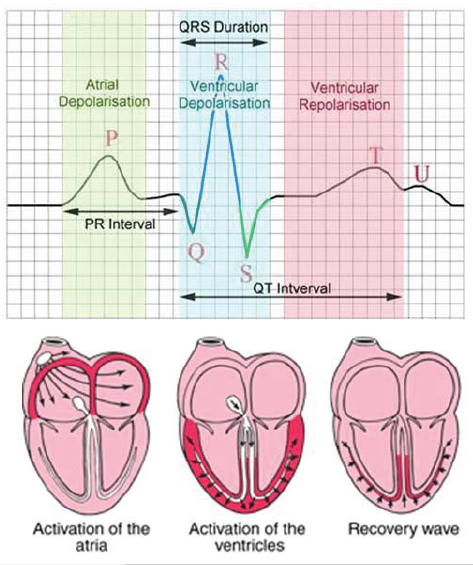
\includegraphics[scale=0.5]{images/ECG.png}
\\Figure 1. ECG waves specification
\\Source: Adapted from \cite{ECGEventB}
\end{center}


The overall processing of the ECG waves consists of capturing the signals from the sensors, de-noising them, detecting the QRS patterns to detect the heartbeat from them, and finally delineating the wave \cite{ECGsignalprocc}.
As in the EEG, ECGs muscle movements, power line interference (PLI), baseline wandering (BW), and motion artifacts (MA) are factors that create noise and prevent the signal from being correclty analysed. For this reason window functions are used to modify the impulse response of the FIR filters in order to reduce the noise.  After having the signal proccessed, the frequency, the distance, the skewness and the existence of the above resulting waves reveal important facts of the heart condition.


As it is used for medical examinations to evaluate several medical conditions, which make the treatment of ECG signals critical in situations like a stroke. For this reason, its treatment needs to be done in real time. The study made in \cite{ECGsyc} implements a real time monitoring system, using LabView, a medical laboratory toolkit, to treat the heartbeat signals reducing noise and when an anomaly is found an SMS is sent to a designated doctor.


\subsection{Signals Synchronisation and Processing}






\subsubsection{Signals Synchronisation}

{\color{red}TODO : You must present ``Clock Synchronisation'' with respect to each method, language, and/or system given bellow.}

\bigskip

\noindent{\textbf{Reactive Systems.}) Reactive systems are systems that are continuously interacting with the exteral environnement, waiting from outside activation in order to react. "The environment can be some physical devices to be controlled, a human operator, or other reactive systems. These systems receive from the environment input events, and compute the output information, which are finally returned to the environment."\cite{SignalPaper}

\begin{figure}[H]
\centering
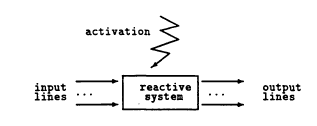
\includegraphics{images/reactive-system.png}
\caption{Reactive Systems. {\color{red}TODO : put the reference for this figure!}}
\end{figure}

The arrival time of events may be different, and the computation needs time. Therefore, it is necessary to follow a correct methodology to implement a reactive system, for example by using synchronization  (synchronous methods), asynchronization (asynchronous methods), or both (GALS are an example).

\smallskip
\noindent{{\textbf{Synchronous Method.}} A way to make programs for reactive system is using synchronous methods. "Synchronous method is an important choice to design these systems, which relies on the synchronous hypothesis. Firstly, the computation time is abstracted as zero, that lets system behaviours be divided into a discrete sequence of instants. At each instant, the system does input-computation output, which takes zero time. Secondly, the different arrival time of events are abstracted as the relative order between events. Even of the physical time is abstracted, the inherent functional properties are not changed, so we can say this method focuses on functional behaviours at a platform-independent level."\cite{SignalPaper} Examples of synchronous languages are : Esterel, Signal, Lustre, which are implementations of the synchronous hypothesis. Synchrounous systems are built using synchronous languages, therefore "each of [the] components of [these systems] receive a common periodic signal (clock) that is used to control its operation and its interaction with other components"\cite{GalsArticle}.

\smallskip
\noindent{{\textbf{Globally-Asynchronous Locally-Synchronous Systems (GALS).}} Synchrounous systems are not efficient when its internal components are not tied to the same clock. A solution is to blend asynchronous solutions with synchronous solutions, this is the purpose of \textit{globally-asynchronous locally-synchronous systems} (GALS), which can be considered  as an optimum middle between synchrounous and asynchrounous systems and as a solution to implement multiclocks systems. 

\smallskip
\noindent{{\textbf{Physically Asynchronous Logically Synchronous (PALS).}} An alternative to GALS are Physically Asynchronous Logically Synchronous Systems (PALS), PALS is a architectural pattern that targets the developpement of Distributed Real-Time Systems (DRTS), the key idea of PALS is to reduce the effort of designing, verifying and implementing DRTS. PALS can be transformed to Real-Time Maude formal specification language by using a formal method\cite{PALSPaper}. There is also a bisimulation theorem "showing that the original synchronous design and the so-called stable states of the corresponding PALS asynchronous design constitute bisimilar systems"\cite{PALSPaper}.

\smallskip
\noindent{{\textbf{Comparison between synchronous languages.}}
The following table compare each synchronous language with a set of specifications. All of these languages can be used to build both synchronous system and GALS.

\begin{table}[H]
\begin{adjustbox}{width=\columnwidth,center}
\begin{tabular}{|l|l|l|l|l|l|l|l|}
\hline
        & Specification language & Programming approach                                                               & Language of compilation & Compile to f. state-machine & Formal semantic & Formal verification & Multi clock \\ \hline
Esterel & Yes                    & Imperative, set of rules                                                           & C                       & Yes                         & Yes             & Yes                 & No          \\ \hline
Signal  & Yes                    & Declarative, data flow                                                             & ?                       & ?                           & Yes             & Yes                 & No?         \\ \hline
Lustre  & Yes                    & \begin{tabular}[c]{@{}l@{}}Declarative, data flow,\\ set of equations\end{tabular} & C                       & Yes                         & Yes             & Yes                 & Yes         \\ \hline
SystemJ & Yes                    & Declarative, data flow                                                             & Java                    & No?                         & Yes             & Yes                 & Yes         \\ \hline
\end{tabular}
\end{adjustbox}
\caption{\color{red} TODO : Give a caption for this Table!}
\end{table}



\subsubsection{Signal Processing}
TBC!



\section{State of the Art}
\subsection{AI for MDE/DSL}
In this part we will discuss the question : how to find the best model using artificial intelligence? This involves a combination of approaches, including, respectively, (i) model-based machine learning (ML); (ii) incremental learning methods; and, (iii) the integration of machine learning into domain modeling. We give below detailed presentation of those approaches : 

\smallskip
\noindent  \textbf{Model-based machine learning.}  involves specifying ML problems using a dedicated modeling language and generating the corresponding ML code automatically, allowing for the creation of highly tailored models for specific scenarios and rapid prototyping and comparison of alternative models\cite{evolutionMDE}. In \cite{mdApproach} a new approach is presented. It is based on the domain-specific modeling (DSM) methodology and involves the creation of a domain-specific modeling language (DSML) that can be used to generate ML models as well as code for their implementation.

\smallskip
\noindent  \textbf{Incremental learning methods.} such as those based on Hoeffding bounds and Hoeffding trees, have been proposed as a way to efficiently process and analyze massive data streams in real-time\cite{evolutionMDE}. 


\smallskip
\noindent  \textbf{The integration of machine learning into domain modeling.}  involves decomposing ML into small, reusable units called microlearning units \cite{evolutionMDE}, which can be modeled and used alongside domain data, allowing for the flexible combination of learned behaviors and domain knowledge. An example of machine learning integration is given in the paper ThingML \cite{ThingML}.  ThingML is an open source MDE solution for CPS and IoT systems that uses a domain-specific modeling language, methodology, and tool to allow for the specification of distributed systems using components, composite state machines, and an action language. The paper proposes the integration of Machine Learning (ML) into the ThingML approach in order to enable the development of data-driven behavior in Cyber-Physical System (CPS) and IoT systems. Finally,the availability of large and high-quality datasets, such as the ModelSet dataset \cite{modelset}, is crucial for the application of machine learning in model-driven engineering.


Machine learning (ML) is a widely used approach for enabling computers to learn from and make decisions based on data. There are many tools and frameworks available for implementing ML algorithms, such as TensorFlow, GraphLab, and Infer.NET. These tools allow for the expression of ML algorithms at a higher level of abstraction, and often include an execution engine for running the algorithms on a variety of devices.
There is also a growing trend towards using a model-based approach for ML, in which ML problems are specified using a dedicated modeling language and the corresponding ML code is generated automatically. This allows for the creation of highly tailored models for specific scenarios and rapid prototyping and comparison of alternative models.
Incremental learning methods, such as those based on Hoeffding bounds and Hoeffding trees \cite{evolutionMDE}, have been proposed as a way to efficiently process and analyze massive data streams in real-time. Tools like MOA provide implementation and support for these methods.
Other research has focused on weaving ML into domain modeling, allowing ML algorithms to be seamlessly integrated into the process of creating models for a particular domain or application. This approach involves decomposing ML into small, reusable units called microlearning units, which can be modeled and used alongside domain data. This approach allows for the flexible combination of learned behaviors and domain knowledge, and can be more accurate and efficient than learning global behaviors. In this same paper \cite{evolutionMDE}, the authors propose a method for seamlessly integrating machine learning into domain modeling by decomposing machine learning into microlearning units that are modeled together with and at the same level as the domain data. The approach is demonstrated using a smart grid case study, showing that it can be significantly more accurate than learning a global behavior, while still being fast enough for live learning.\\


The application of machine learning (ML) to software engineering has gained significant attention in recent years, with a focus on three types of ML models: code-generating models, representational models of code, and pattern mining models. These models have various applications, such as code recommendation systems, inferring coding conventions, clone detection, and code-to-text and text-to-code translation.There are several existing datasets related to software models, including the LindholmenDataset and ModelSet, as well as datasets of OCL expressions, BPMN models, and APIs classified using Maven Central tags. However, many of these datasets have limitations, such as a variety of formats and versions, invalid or poor quality models, or a lack of labels.
There have been several studies on the application of AI and ML to address MDE problems, including search-based algorithms and reinforcement learning for co-evolution and model repair, respectively. There have also been efforts to classify UML class diagrams and Ecore meta-models, and to use clustering techniques on collections of models. However, many of these studies are not easily replicable due to the lack of available datasets or the difficulty in processing the models.
ModelSet dataset, which includes over 10,000 labeled models, aims to address the need for a large and high-quality dataset of software models for use in ML research. The dataset is composed of models in the Ecore metamodeling language, and includes labels for the model category and domain, as well as structural and textual features. The paper \cite{modelset} demonstrates the use of the dataset in a classification task, showing that it can be used to improve the accuracy of existing ML models for classifying Ecore models.\\


The paper \cite{mdApproach} proposes a novel approach to integrating machine learning (ML) models with software and systems engineering models, particularly in the context of model-driven software engineering (MDSE). The approach is based on the domain-specific modeling (DSM) methodology and involves the creation of a domain-specific modeling language (DSML) that can be used to generate ML models as well as code for their implementation. The DSML is demonstrated through a case study in the Internet of Things (IoT) and cyber-physical systems domains, but is not limited to these specific verticals.
There are several directions for future work, including the support of semi-supervised ML, the extension of the supported ML methods to include kernel methods and advanced artificial neural network architectures, the addition of more target platforms and programming languages, and the inclusion of advanced autoML functionalities.

Domain analysis \cite{mdApproachMonitoring}  is about studying and understanding a particular problem or domain in order to develop a solution or model that can effectively solve the problem. In the context of machine learning, domain analysis involves understanding the properties of the data, the target variables, and the relationships between the observed and target variables, in order to develop a model using techniques such as supervised learning. However, in non-stationary environments, the joint probability distribution between the observed and target variables may change over time, leading to differences between the training and test sets, which may affect the performance of the model. To address this problem, researchers have developed methods that adapt to non-stationary environments, such as online learning algorithms or hybrid approaches.

The domain meta-model refers to the larger system that is required to effectively apply machine learning techniques in a commercial setting, considering factors such as latency, cost, compatibility, and scalability. The domain meta-model also needs to consider the process of continuous learning, which involves regularly updating the model with new data in order to maintain its performance. \\


The Internet of Things (IoT) is a network of interconnected devices that can communicate with each other and with external systems. Cyber-Physical Systems (CPS) are systems of systems that combine both physical and virtual elements. Artificial Intelligence (AI) is increasingly being used in the development of IoT and CPS systems to enable them to have cognitive capabilities such as learning. Model-Driven Engineering (MDE) is a promising approach that provides both abstraction and automation for the specification, design, development, analysis, verification and maintenance of CPS and IoT systems. ThingML \cite{ThingML} is an open source MDE solution for CPS and IoT systems that uses a domain-specific modeling language, methodology and tool to enable the specification of distributed systems using components, composite state machines and an action language. 

In the field of IoT, the increasing number of connected devices has led to the need for efficient network management schemes. Hierarchical network architectures such as H-CRANs and cooperative cloud-edge computing have been developed to provide efficient network-wide management and address the computing demands of IoT devices. Edge computing, in particular, has emerged as a way to process tasks at the network edge near mobile users in order to reduce latency and improve service quality for delay-sensitive applications. To minimize delay in mobile computing networks, various approaches have been proposed, such as task offloading, content caching, and reducing data exchange among IoT systems. Machine learning can also be used to improve computing performance by adapting service provisioning based on past events. In the article \cite{DelaySensitiveIoT}, a decision tree model was proposed to classify tasks as delay-sensitive or delay-insensitive, and a priority queuing model was introduced to prioritize delay-sensitive tasks in order to avoid long queuing delays. The decision tree model was trained and tested using simulated data sets, and the accuracy of the model was investigated. The proposed model was shown to effectively classify tasks and reduce queuing delay in the edge device.


\subsection{MDE/DSL for AI}
The different notions of models in AI and MDE brings some difficulty in integrating these two domain together. ML models or techniques as mentioned before are completely distinct than the models used in MDE; one is a statistical model while another is a structural model. Even though the terminology of the model-based ML exists in the domain, this refers to the capability of the models to function without the need of the training datasets. This is contrary to the instance-based models, which requires some part of the observed dataset even once the training phase is done. However, these two terms however seems to have a nuanced notion after the emergence of the term model-based in Infer.Net \cite{inferNet}. The notion model-based ML thereafter can be used to refer to any of these term: instance-based or model based architecture.

As mentioned in \cite{mdApproach}, the notion of models in the Data Analytics and Machine Learning(DAML) community is completely different than the one in Software and System Engineering(SSE). A model in the DAML community is more an abstraction to the values inside the datasets rather than the architecture of the datasets itself. For example, a statistical model in DAML is a model defining the probability distribution in the dataset and a feature-based models represents the summarization or the approximation of the data instances. In this Machine Learning era, most of the ML models used : Support Vector Machine(SVM), Artifical Neural Network(ANN), Probabilistic Graphical Models(PGM) or Bayesian Deep Learning are among the models that characterise the observed datas from the analytics perspective. 

The two main principles of MDE is to provide a level of abstraction in order to hide the complexity behind a model and providing a partial or full automation of the transformations needed in the system, such as model-to-text for code generation or model-to-model for transferring current model to another system. These two principles can be found in the existing libraries or frameworks in the ML domain, for example with Tensorflow \cite{tensorflow} which provides a powerful API using advanced implemented technique, Keras \cite{keras} which add another layer of abstraction allowing the use of the APIs of Tensorflow and other API frameworks e.g. PlaidML \cite{plaidML}, or with the workflow designers: KNIME \cite{knime} and RapidMiner \cite{rapidminer} and visualization toolkits: TensorBoard \cite{tensorboard}, which allows a graphical user interface instead of using code. 
However, these libraries or frameworks are not conformed to the holistic approach introduced in MDSE, where the models need to also includes the information about the entire application, and the code generation should be able to generate the software implementation with the code.

Moreover, the abstraction of the functionalities of these frameworks and libraries are further explored by the idea of Model-Interchange Formats, e.g. Predictive Model Language(PMML) \cite{pmml}, Portable Format for Analytics(PFA) \cite{pfa} and Open Neural Network Exchange(ONNX) \cite{onnx}. The code generation of a ML models are also explored by the Infer.Net \cite{inferNet} by using the PGMs as a MDSE model therefore allowing a whole software implementation in C\# from the model. However, as Infer.Net only use PGMS as its source, there may be shortcomings in terms of expressiveness for the whole software system. The approach by ML-Quadrat \cite{mdApproach}, \cite{ThingML}, based on ThingML(a modelling language specifically for Internet of Things (IoT)) is the nearest technology found to be implementing the holistic nature of the MDSE. This technology are looking forward to create a synergy between the two different notion of models, allowing a more seamless model engineering in these two domains.

% Please add the following required packages to your document preamble:
\begin{table}[]
\begin{adjustbox}{width=\columnwidth,center}
\begin{tabular}{@{}|l|l|l|l|l|@{}}
\toprule
Description                    & Technologies            & Full-code generation      & DAML-support              & Model Type           \\ \midrule
ML libraries \& frameworks     & TensorFlow, Keras, etc. &                           & \ding{51} & DAML models          \\ \midrule
DAML workflow designers        & KNIME, RapidMiner, etc. &                           & \ding{51} & DAML models          \\ \midrule
Model Interchange Formats(MIF) & PMML,PFA,ONNX           &                           & \ding{51} & DAML models          \\ \midrule
'Model-based' ML               & Infer.Net               & \ding{51} & \ding{51} & SE \& ML(PGM) models \\ \midrule
MDE4IOT + ML                   & ML-Quadrat              & \ding{51} & \ding{51} & SE \& DAML models    \\ \bottomrule
\end{tabular}
\end{adjustbox}
\caption{\label{MDE4AI-table}Comparison in features provided by each related works mentioned.}
\end{table}




\section{Case Studies}


\subsection{Application domains}

\bibliographystyle{plain}
\bibliography{references}
\end{document}  
